% ---------------------------------------------------------------- 13
\begin{frame}{Vocabulaire : quatre objets, un raisonnement}
\begin{center}
{\setlength{\tabcolsep}{3pt}\begin{tabular}{@{}p{2.0cm}p{2.5cm}p{4.2cm}p{4.3cm}@{}}
\toprule
\textbf{Objet} & \textbf{Notation} & \textbf{Interprétation} & \textbf{Exemple (pièce biaisée)} \\
\midrule
A priori & $p(\theta)$ & ce que l'on croit \emph{avant} les données &
Beta$(2,2)$ : « la pièce est plausiblement équilibrée » \\[2mm]
Vraisemblance & $p(y \given \theta)$ & probabilité des données \emph{si} le paramètre valait $\theta$ &
Bin$\big(10, \theta\big)$ : 7 faces sur 10 \\[2mm]
A posteriori & $p(\theta \given y)$ & la croyance \emph{après} les données &
Beta$(9,5)$ : centré sur 0,64 \\[2mm]
Prédictive & $p(\tilde y \given y)$ & ce qu'on attend de la prochaine observation &
$P(\text{face}) = \int \theta\, p(\theta \given y)\,\mathrm{d}\theta = 0{,}643$ \\
\bottomrule
\end{tabular}}
\end{center}
\vspace{1mm}
\begin{kbox}[La règle d'or]
Le prior est \textbf{ce qu'on met sur la table} ; le posterior est
\textbf{ce qui en reste après avoir vu les données}. Rien ne se perd, tout se met à jour.
\end{kbox}
\end{frame}

% ---------------------------------------------------------------- 14
\begin{frame}{Exemple fondateur : la pièce truquée --- l'énoncé}
\begin{ebox}[Énoncé]
On lance 10 fois une pièce et on obtient \textbf{7 faces}.
\begin{itemize}
  \item Paramètre : $\theta = P(\text{face}) \in [0,1]$
  \item Prior : $\theta \sim \mathrm{Beta}(1,1)$ (uniforme)
  \item Vraisemblance : $y \given \theta \sim \mathrm{Bin}(10, \theta)$
\end{itemize}
\vspace{1mm}
\textbf{Questions}
\begin{enumerate}
  \item Forme du posterior ?
  \item Valeur centrale ?
  \item Intervalle de crédibilité à 95 \% ?
  \item $P(\theta > 0{,}5 \given y)$ ?
\end{enumerate}
\end{ebox}
\end{frame}

% [split]
\begin{frame}{Exemple fondateur : la pièce truquée --- le posterior}
\begin{center}
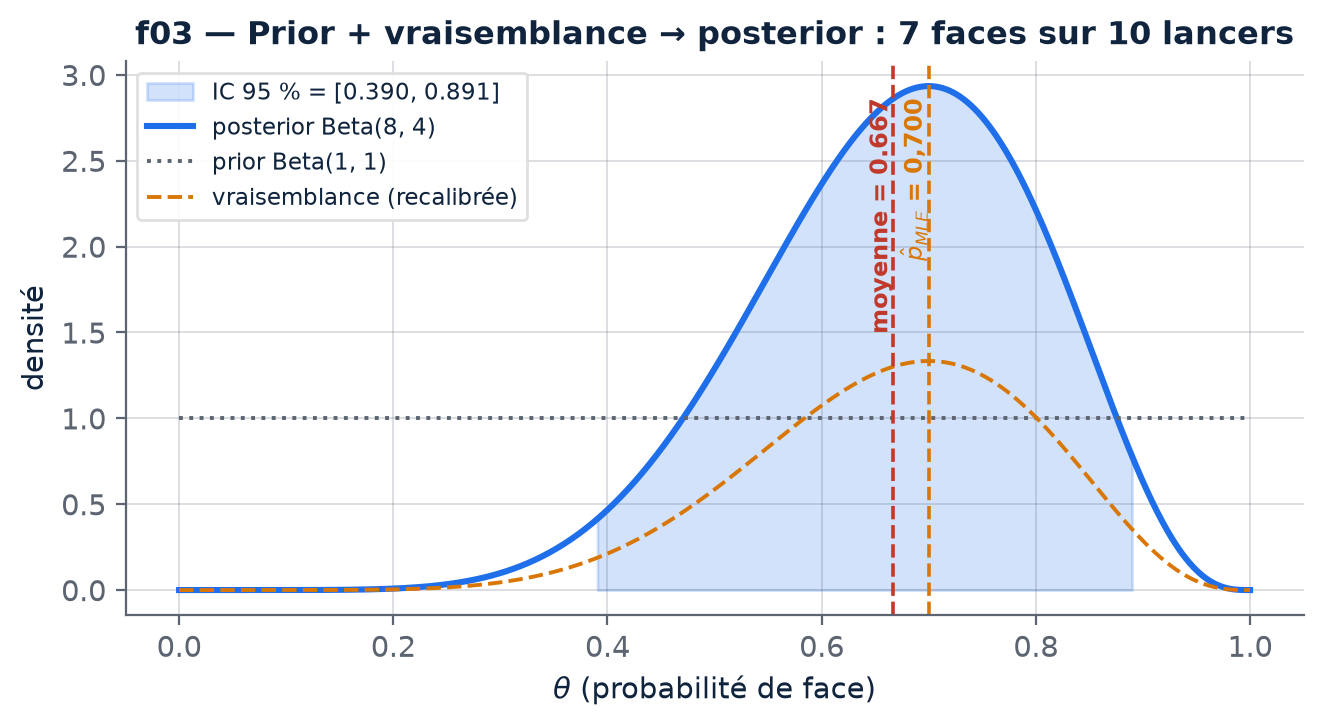
\includegraphics[width=.86\textwidth]{f03_piece_posterior.png}
\end{center}
\end{frame}

% [split]
\begin{frame}{Exemple fondateur : la pièce truquée --- le posterior}

\vspace{-1mm}
\begin{solbox}[Résultats calculés (script \file{src/fig\_ch1.py}, exécuté)]
\centering\small
posterior $\mathrm{Beta}(8,4)$ \quad|\quad moyenne $0{,}667$ \quad|\quad mode $0{,}700$
\quad|\quad IC 95 \% $[0{,}390 \,;\, 0{,}891]$ \quad|\quad $P(\theta > 0{,}5 \given y) = 0{,}887$
\end{solbox}
\end{frame}

% ---------------------------------------------------------------- 15
% [suite]
\begin{frame}{Comment lire un résultat bayésien}
\begin{columns}[t]
\begin{column}{0.5\textwidth}
\begin{kbox}[Trois nombres]
\begin{itemize}
  \item \textbf{Moyenne a posteriori} $0{,}667$ : minimise l'erreur quadratique,
        c'est l'estimateur par défaut.
  \item \textbf{Médiane} : robuste, sert au calcul du HDI.
  \item \textbf{Mode (MAP)} $0{,}700$ : coïncide ici avec le maximum de vraisemblance.
        Avec un prior asymétrique, il s'en écarte — c'est le \emph{shrinkage}.
\end{itemize}
\end{kbox}
\end{column}
\begin{column}{0.47\textwidth}
\begin{solbox}[Intervalle de crédibilité 95 \%]
$[0{,}390 \,;\, 0{,}891]$

\vspace{1.5mm}
\small « Il y a 95 \% de chance que la vraie probabilité de face soit dans cet intervalle,
\textbf{compte tenu du prior et des 7 faces observées}. »

\vspace{1.5mm}
Variante HDI (le plus court des intervalles de masse 0,95) : $[0{,}412 \,;\, 0{,}906]$ ---
légèrement plus court que l'intervalle à queues égales.
\end{solbox}
\end{column}
\end{columns}
\vspace{1mm}
\begin{ebox}[Effet mesurable du prior, mêmes données]
Avec $\theta \sim \mathrm{Beta}(2,2)$ au lieu de Beta$(1,1)$ : posterior $\mathrm{Beta}(9,5)$,
moyenne $0{,}643$, IC 95 \% $[0{,}386 \,;\, 0{,}861]$.
Le prior a ramené la croyance de 0,667 vers 0,643 : c'est le \textbf{\textit{shrinkage}}.
\end{ebox}
\vspace{1mm}
\end{frame}

% [suite]
\begin{frame}{Comment lire un résultat bayésien (suite)}
\begin{wbox}[À ne jamais écrire]
\nok{} « Il y a 95 \% de chance que la vraie valeur soit dans \emph{l'intervalle de confiance
fréquentiste} » \;; \;
\nok{} « $p(\theta) = 0{,}667$ est la probabilité que $\theta$ vaille exactement 0,667 »
(probabilité d'un point : nulle pour une loi continue).
\end{wbox}
\end{frame}

% ---------------------------------------------------------------- 16
\begin{frame}{Animation : mise à jour, observation après observation}
% [rogna]
\small
\begin{columns}[t]
\begin{column}{0.56\textwidth}
\begin{center}
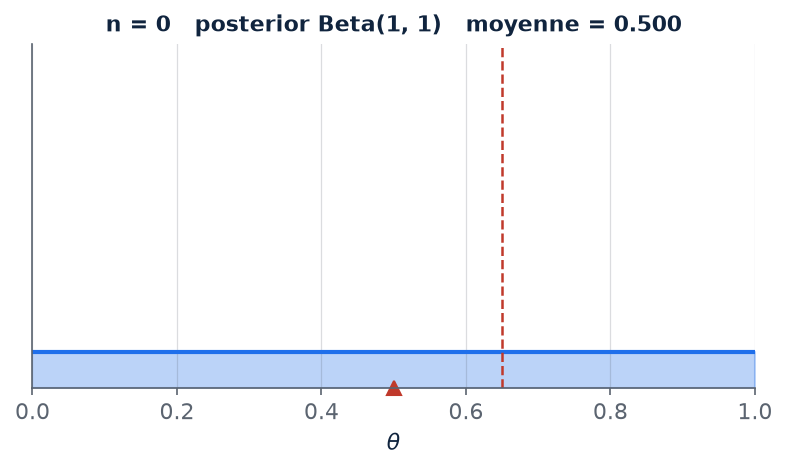
\includegraphics[width=\textwidth]{f04_frames/frame-0.png}
\end{center}
\vspace{-2mm}
\centering\footnotesize
\begin{tabular}{@{}llll@{}}
\toprule
$n$ & faces observées & posterior & moyenne \\
\midrule
0 (prior) & 0 & Beta$(1,1)$ & 0,500 \\
1 & 1 & Beta$(2,1)$ & 0,667 \\
5 & 5 & Beta$(6,1)$ & 0,857 \\
20 & 16 & Beta$(17,5)$ & 0,773 \\
200 & 121 & Beta$(122,80)$ & 0,604 \\
\bottomrule
\end{tabular}
\end{column}
\begin{column}{0.42\textwidth}
\begin{abox}[À faire devant la classe]
Ouvrir \file{notebooks/TP1\_mise\_a\_jour\_\allowbreak bayesienne.ipynb} et rejouer l'animation
($\alpha$, $\beta$ modifiables).

\vspace{1.5mm}
\textbf{Question :} à partir de quel $n$ une observation supplémentaire
déplace-t-elle la moyenne de moins de 0,005 ?
\end{abox}
\vspace{1mm}
\begin{ebox}[Réponse (calculée)]
Pour la réalisation simulée à $n = 200$, l'écart-type du posterior vaut $0{,}034$
et la moyenne ne bouge que de $\approx 0{,}002$ par nouvelle observation.
$5$ faces sur les $5$ premiers lancers donnaient 0,857 : \textbf{le petit échantillon
est extrême}, l'information ne s'achète pas, elle s'accumule en $1/\sqrt{n}$.
\end{ebox}
\end{column}
\end{columns}
\end{frame}

% ---------------------------------------------------------------- 17
% [split]
\begin{frame}{Application : sondage électoral}
\begin{center}
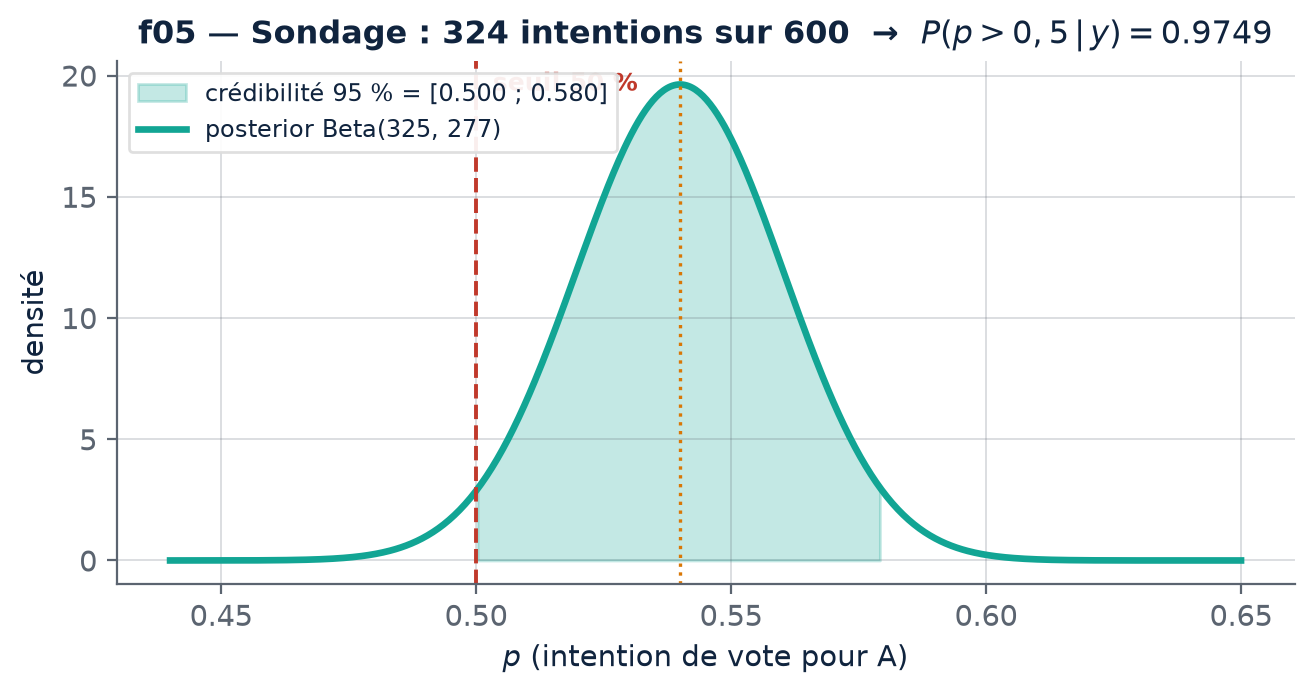
\includegraphics[width=\textwidth]{f05_sondage_posterior.png}
\end{center}
\end{frame}

% [split]
% [suite5]
\begin{frame}{Application : sondage électoral}
\begin{columns}[t]
\begin{column}{0.48\textwidth}
\begin{ebox}[Données]
$n = 600$ personnes interrogées, \textbf{324} intentions de vote pour A (54,0 \%).
Prior Beta$(1,1)$.
\end{ebox}
\begin{solbox}[Ce qu'on peut dire]
\begin{itemize}
  \item Posterior : $\mathrm{Beta}(325, 277)$, moyenne $0{,}540$
  \item Crédibilité 95 \% : $[0{,}500 \,;\, 0{,}580]$
  \item \textbf{$P(p > 0{,}5 \given y) = 0{,}975$}
  \item $P(p > 0{,}52) = 0{,}836$ \quad (intérêt : la marge d'un second tour)
  \item $P(p > 0{,}55) = 0{,}310$ \quad (le candidat est loin d'être certain de passer)
\end{itemize}
\end{solbox}
\end{column}
\end{columns}
\end{frame}

% [suite5]
\begin{frame}{Application : sondage électoral (suite)}
\begin{kbox}[L'avantage décisif]
Le fréquentiste donne $[0{,}50 \,;\, 0{,}58]$ mais ne peut pas répondre à
« le candidat A est-il \emph{probablement} au-dessus de 50 \% ? ».
Le bayésien répond : \textbf{97,5 \%}.
\end{kbox}
\end{frame}

% ---------------------------------------------------------------- 18
\begin{frame}{Pièges de lecture des intervalles}
\begin{columns}[t]
\begin{column}{0.49\textwidth}
\begin{wbox}[Intervalle de confiance fréquentiste]
\begin{itemize}
  \item Construit sur la variabilité de $\hat p$.
  \item \textbf{Ce dont on est sûr :} si l'on répétait l'étude un très grand nombre de fois,
        alors 95 \% des intervalles ainsi construits contiendraient $p$.
  \item \textbf{Ce dont on n'est pas sûr :} que \emph{cet} intervalle contienne $p$.
  \item Il ne peut pas devenir plus étroit quand on dispose d'information externe
        \emph{à moins} de changer la méthode.
\end{itemize}
\end{wbox}
\end{column}
\begin{column}{0.49\textwidth}
\begin{solbox}[Intervalle de crédibilité bayésien]
\begin{itemize}
  \item Construit sur la variabilité de $\theta$.
  \item \textbf{Ce dont on est sûr :} $P(\theta \in [a,b] \given y) = 0{,}95$.
  \item Il \textbf{rétrécit} mécaniquement si l'on ajoute de l'information externe
        justifiée (les priors conjugués du chapitre 2).
  \item Variante HDI : l'intervalle \emph{le plus court} de masse 0,95
        (chapitre 3, slide sur HDI contre queue égale).
\end{itemize}
\end{solbox}
\end{column}
\end{columns}
\vspace{1mm}
\centering\small
Les deux intervalles se ressemblent numériquement quand $n$ est grand —
ils \textbf{ne racontent pas la même chose}.
\end{frame}
